% Created 2019-12-26 Thu 02:52
% Intended LaTeX compiler: pdflatex
\documentclass[11pt]{article}
\usepackage[utf8]{inputenc}
\usepackage[T1]{fontenc}
\usepackage{graphicx}
\usepackage{grffile}
\usepackage{longtable}
\usepackage{wrapfig}
\usepackage{rotating}
\usepackage[normalem]{ulem}
\usepackage{amsmath}
\usepackage{textcomp}
\usepackage{amssymb}
\usepackage{capt-of}
\usepackage{hyperref}
\usepackage{minted}
\author{Tigany Zarrouk}
\date{\today}
\title{Final Ti Model Results}
\hypersetup{
 pdfauthor={Tigany Zarrouk},
 pdftitle={Final Ti Model Results},
 pdfkeywords={},
 pdfsubject={},
 pdfcreator={Emacs 26.3 (Org mode 9.1.9)}, 
 pdflang={English}}
\begin{document}

\maketitle
\tableofcontents



\section{Objective Function}
\label{sec:org3d1ac89}


PARAMETERS
  fdd=0.1958363809 qdds=0.5591275855 qddp=0.5690351902 qddd=0.7745947522 b0=58.0906936439 p0=1.2185323579 b1=-3.2299188646 p1=0.6862915307 b2=593519.1134129359 m2=-11.5000000000 p2=0.0000000000 ndt=2.0000000000 cr1=-6.0000000000 cr2=3.0474400934 cr3=-1.2317472193 r1dd=6.5000000000 rcdd=10.0000000000 rmaxhm=10.1000000000 npar=18 
VARGS
    -vfdd=0.1958363809 -vqdds=0.5591275855 -vqddp=0.5690351902 -vqddd=0.7745947522 -vb0=58.0906936439 -vp0=1.2185323579 -vb1=-3.2299188646 -vp1=0.6862915307 -vb2=593519.1134129359 -vm2=-11.5000000000 -vp2=0.0000000000 -vndt=2.0000000000 -vcr1=-6.0000000000 -vcr2=3.0474400934 -vcr3=-1.2317472193 -vr1dd=6.5000000000 -vrcdd=10.0000000000 -vrmaxhm=10.1000000000 



\begin{center}
\begin{tabular}{lrr}
Quantity & From Model & Target\\
\hline
a\(_{\text{hcp}}\) & 5.58523112 & 5.57678969\\
c/a & 1.58371266 & 1.58731122\\
a\(_{\text{omega}}\) & 8.93475285 & 8.73254342\\
c\(_{\text{omega}}\) & 5.38726911 & 5.32343103\\
a\(_{\text{4h}}\) & 5.57584691 & 5.56325146\\
c\(_{\text{4h}}\) & 18.09810672 & 17.75908031\\
a\(_{\text{6h}}\) & 5.57365569 & 5.54639384\\
c\(_{\text{6h}}\) & 27.18378460 & 26.77136353\\
a\(_{\text{bcc}}\) & 6.20079768 & 6.17948863\\
a\(_{\text{fcc}}\) & 7.87290654 & 7.88677000\\
DE(o,h) & 0.58764167 & -0.63343333\\
DE(4h,h) & 1.58019500 & 3.17160000\\
DE(6h,h) & 2.48264833 & 3.72005000\\
DE(b,h) & 5.35128500 & 7.63520000\\
DE(f,h) & 3.78088500 & 4.51880000\\
c\(_{\text{11}}\) & 171.60928873 & 176.10000000\\
c\(_{\text{33}}\) & 198.90063708 & 190.50000000\\
c\(_{\text{44}}\) & 47.42549704 & 50.80000000\\
c\(_{\text{12}}\) & 94.65941969 & 86.90000000\\
c\(_{\text{13}}\) & 61.22624060 & 68.30000000\\
M\(_{\text{freq}}\)\(_{\text{0}}\) & 2.59341377 & 2.85858719\\
M\(_{\text{freq}}\)\(_{\text{1}}\) & 2.59341378 & 2.85858719\\
M\(_{\text{freq}}\)\(_{\text{2}}\) & 2.59341378 & 2.85858719\\
M\(_{\text{freq}}\)\(_{\text{3}}\) & 2.59341379 & 2.85858719\\
M\(_{\text{freq}}\)\(_{\text{4}}\) & 5.85272461 & 5.66706047\\
M\(_{\text{freq}}\)\(_{\text{5}}\) & 5.85272461 & 5.66706047\\
H\(_{\text{freq}}\)\(_{\text{0}}\) & 3.82320403 & 4.80643423\\
H\(_{\text{freq}}\)\(_{\text{1}}\) & 3.82320403 & 5.58010025\\
H\(_{\text{freq}}\)\(_{\text{2}}\) & 6.40288977 & 5.65316738\\
H\(_{\text{freq}}\)\(_{\text{3}}\) & 6.40288977 & 6.36651842\\
H\(_{\text{freq}}\)\(_{\text{4}}\) & 7.92857431 & 6.40050186\\
H\(_{\text{freq}}\)\(_{\text{5}}\) & 7.92857431 & 7.64082373\\
bandw.  G & 3.69394702 & 5.87085872\\
bandw.  K & 4.65178817 & 4.97424321\\
bandw.  M & 5.19329495 & 7.78109872\\
bandw.  L & 4.21232412 & 6.34433701\\
bandw.  H & 3.54700549 & 9.70902614\\
DOSerr\(_{\text{h}}\) & 0.00000000 & 0.00000000\\
DOSerr\(_{\text{o}}\) & 0.00000000 & 0.00000000\\
E\(_{\text{pris}}\)\(_{\text{f}}\) & 98.95340236 & 220.00000000\\
\end{tabular}
\end{center}



----------     E\(_{\text{prismatic}}\)\(_{\text{fault}}\)     -----------

\begin{center}
\begin{tabular}{lrll}
tbe: & 98.953 & mJ/m\(^{\text{2}}\) & \\
DFT: & 250.000 & mJ/m\(^{\text{2}}\) & [Benoit  2012]\\
DFT: & 233.000 & mJ/m\(^{\text{2}}\) & [Ackland 1999]\\
\end{tabular}
\end{center}


----------     E\(_{\text{Basal}}\)\(_{\text{fault}}\) I2     -----------

\begin{center}
\begin{tabular}{lrll}
tbe: & 211.658 & mJ/m\(^{\text{2}}\) & \\
DFT: & 260.000 & mJ/m\(^{\text{2}}\) & [Benoit  2012]\\
\end{tabular}
\end{center}

\section{Defect Clusters}
\label{sec:orge32534c}

----------     E\(_{\text{vacancy}}\)\(_{\text{formation}}\)     ----------

\begin{center}
\begin{tabular}{lll}
tbe: & 2.347  eV & \\
DFT: & 1.950  eV & GGA-PAW:   Angsten  (2013)\\
exp: & 1.270  eV & Hashimoto  (1984)\\
\end{tabular}
\end{center}

\subsection{Octahedral O interstitial relaxation}
\label{sec:orgf765251}

Initial:
\begin{center}
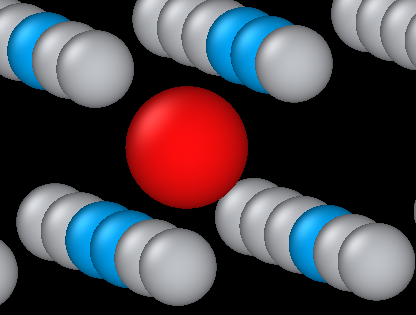
\includegraphics[width=.9\linewidth]{Images/initial_octahedral_ox_ovito.png}
\end{center}

Final:
\begin{center}
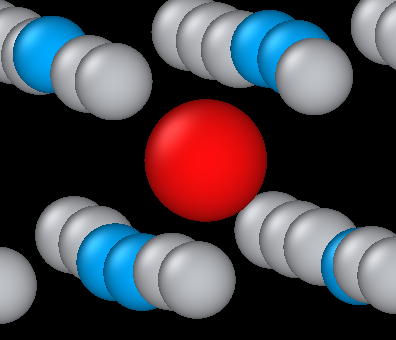
\includegraphics[width=.9\linewidth]{Images/final_octahedral_ox_ovito.png}
\end{center}

\subsection{Tetrahedral O interstitial relaxation}
\label{sec:orgd0b508f}

Initial:
\begin{center}
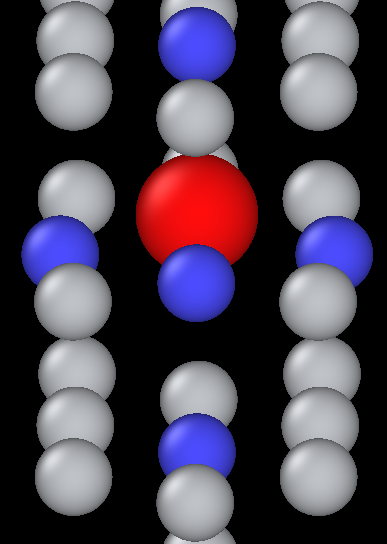
\includegraphics[width=.9\linewidth]{Images/final_model_final_tetra_ox.png}
\end{center}

Final:
\begin{center}
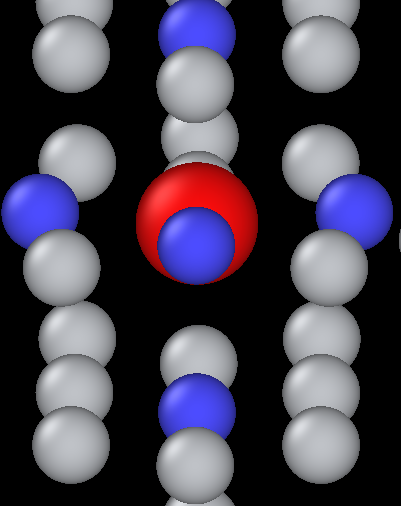
\includegraphics[width=.9\linewidth]{Images/final_model_initial_tetra_ox_ovito.png}
\end{center}

\subsection{Energies for defects}
\label{sec:org97740cc}

Relative differences are 

>> (E\(_{\text{tetrahedral}}\) - E\(_{\text{octahedral}}\)) 
\begin{center}
\begin{tabular}{lll}
tbe: & 1.65 eV & \\
GGA-DFT: & 1.23 eV & Kwasniak (2013)\\
\end{tabular}
\end{center}

>> (E\(_{\text{hexahedral}}\) - E\(_{\text{octahedral}}\))
\begin{center}
\begin{tabular}{ll}
tbe: & 0.90 eV\\
\end{tabular}
\end{center}

> Note: Preference for tetrahedral oxygen to go into hexahedral site as seen by images above

All formation energies below use the chemical potential of Akysonov
(2013) of value \(\mu_{\text{oxygen}} = \frac{5.6}{ 2} eV\).

\subsection{All formation energies}
\label{sec:org6711a4b}

\begin{center}
\begin{tabular}{ll}
Quantity & Energy (eV)\\
\hline
Ef\(_{\text{Vf}}\) & 2.347\\
 & \\
Ef\(_{\text{T}}\)\(_{\text{sol}}\) & -  21.783\\
Ef\(_{\text{T}}\)\(_{\text{dil}}\)\(_{\text{imp}}\) & -  28.991\\
Ef\(_{\text{T}}\)\(_{\text{formation}}\) & -  21.783\\
Ef\(_{\text{T}}\)\(_{\text{V}}\)\(_{\text{formation}}\) & -  18.905\\
Ef\(_{\text{T}}\)\(_{\text{vac}}\)\(_{\text{sol}}\)\(_{\text{bind}}\) & -   0.530\\
 & \\
Ef\(_{\text{O}}\)\(_{\text{sol}}\) & -  23.436\\
Ef\(_{\text{O}}\)\(_{\text{dil}}\)\(_{\text{imp}}\) & -  30.645\\
Ef\(_{\text{O}}\)\(_{\text{formation}}\) & -  23.436\\
Ef\(_{\text{O}}\)\(_{\text{V}}\)\(_{\text{formation}}\) & -  18.905\\
Ef\(_{\text{O}}\)\(_{\text{vac}}\)\(_{\text{sol}}\)\(_{\text{bind}}\) & -   2.183\\
 & \\
Ef\(_{\text{OO}}\)\(_{\text{sol}}\) & -  49.606\\
Ef\(_{\text{OO}}\)\(_{\text{dil}}\)\(_{\text{imp}}\) & -  56.814\\
Ef\(_{\text{OO}}\)\(_{\text{formation}}\) & -  46.806\\
Ef\(_{\text{OO}}\)\(_{\text{V}}\)\(_{\text{formation}}\) & -  41.910\\
Ef\(_{\text{OO}}\)\(_{\text{vac}}\)\(_{\text{sol}}\)\(_{\text{bind}}\) & -   2.547\\
 & \\
Ef\(_{\text{OOO}}\)\(_{\text{sol}}\) & -  76.037\\
Ef\(_{\text{OOO}}\)\(_{\text{dil}}\)\(_{\text{imp}}\) & -  83.246\\
Ef\(_{\text{OOO}}\)\(_{\text{formation}}\) & -  70.437\\
Ef\(_{\text{OOO}}\)\(_{\text{V}}\)\(_{\text{formation}}\) & -  66.013\\
Ef\(_{\text{OOO}}\)\(_{\text{vac}}\)\(_{\text{sol}}\)\(_{\text{bind}}\) & -   2.076\\
 & \\
Ef\(_{\text{OOOO}}\)\(_{\text{sol}}\) & - 102.470\\
Ef\(_{\text{OOOO}}\)\(_{\text{dil}}\)\(_{\text{imp}}\) & - 109.679\\
Ef\(_{\text{OOOO}}\)\(_{\text{formation}}\) & -  94.070\\
Ef\(_{\text{OOOO}}\)\(_{\text{V}}\)\(_{\text{formation}}\) & -  88.998\\
Ef\(_{\text{OOOO}}\)\(_{\text{vac}}\)\(_{\text{sol}}\)\(_{\text{bind}}\) & -  2.724\\
 & \\
Ef\(_{\text{OOOOO}}\)\(_{\text{sol}}\) & - 128.781\\
Ef\(_{\text{OOOOO}}\)\(_{\text{dil}}\)\(_{\text{imp}}\) & - 135.989\\
Ef\(_{\text{OOOOO}}\)\(_{\text{formation}}\) & - 117.581\\
Ef\(_{\text{OOOOO}}\)\(_{\text{V}}\)\(_{\text{formation}}\) & - 113.649\\
Ef\(_{\text{OOOOO}}\)\(_{\text{vac}}\)\(_{\text{sol}}\)\(_{\text{bind}}\) & - 1.583\\
 & \\
Ef\(_{\text{OOOOOO}}\)\(_{\text{sol}}\) & - 155.148\\
Ef\(_{\text{OOOOOO}}\)\(_{\text{dil}}\)\(_{\text{imp}}\) & - 162.357\\
Ef\(_{\text{OOOOOO}}\)\(_{\text{formation}}\) & - 141.148\\
Ef\(_{\text{OOOOOO}}\)\(_{\text{V}}\)\(_{\text{formation}}\) & - 137.110\\
Ef\(_{\text{OOOOOO}}\)\(_{\text{vac}}\)\(_{\text{sol}}\)\(_{\text{bind}}\) & - 1.690\\
\end{tabular}
\end{center}

\section{Gamma surfaces}
\label{sec:org05faaa1}

Energies are accurate to within 2 mJm\(^{\text{-2}}\), comparing the energies of
points in the corners which (the zeros of energy). So surface energies
might be  \(\pm 2\) mJm\(^{\text{-2}}\) off which is reasonable. 

These calculations were done in tight binding with 15 layers for both
basal and prismatic with k-points adjusted accordingly. 
DFT comparisons are usind results of Rodney. 

The Pyramidal surface was obtained using the same 32 atom cell that
Ready used in his paper on the pyramidal gamma surface with DFT
pseudopotentials. 

\newpage
\subsection{Basal}
\label{sec:org0399a23}

TBE:
\begin{center}
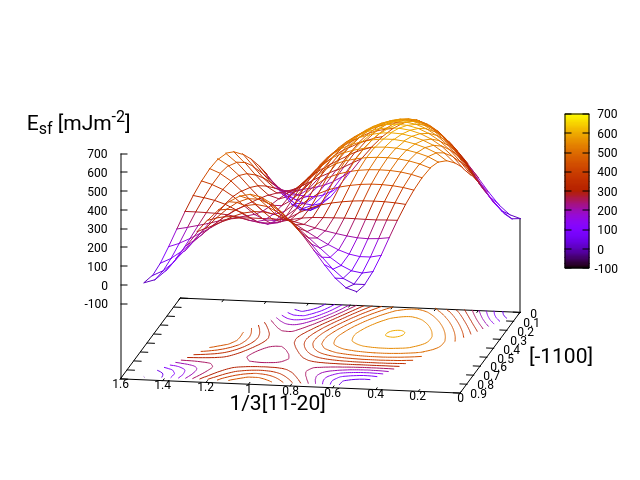
\includegraphics[width=.9\linewidth]{Images/basal_gs_noo_2019-11-08_alat.png}
\end{center}

DFT:
\begin{center}
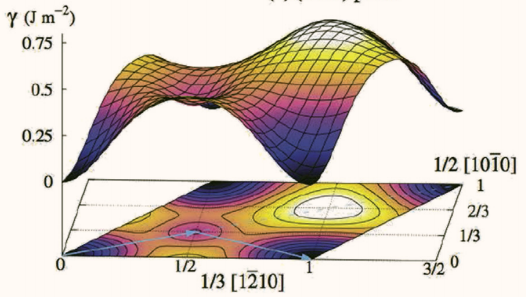
\includegraphics[width=.9\linewidth]{Images/rodney_basal_ti_gamma_surface.png}
\end{center}

\subsection{Prismatic}
\label{sec:org3f22fc3}

TBE:
\begin{center}
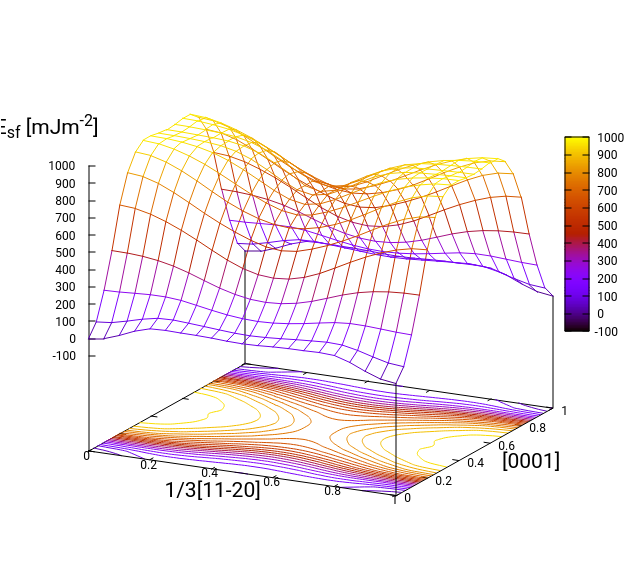
\includegraphics[width=.9\linewidth]{Images/prismatic_gs_noo_2019-11-08_alat.png}
\end{center}

DFT:
\begin{center}
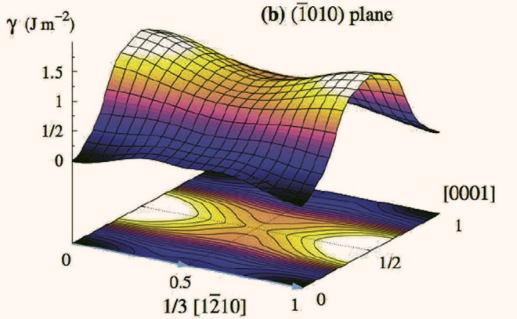
\includegraphics[width=.9\linewidth]{Images/rodney_prismatic_ti_gamma_surface.png}
\end{center}

\subsection{Pyramidal first order}
\label{sec:org1d8a2f6}

TBE:
\begin{center}
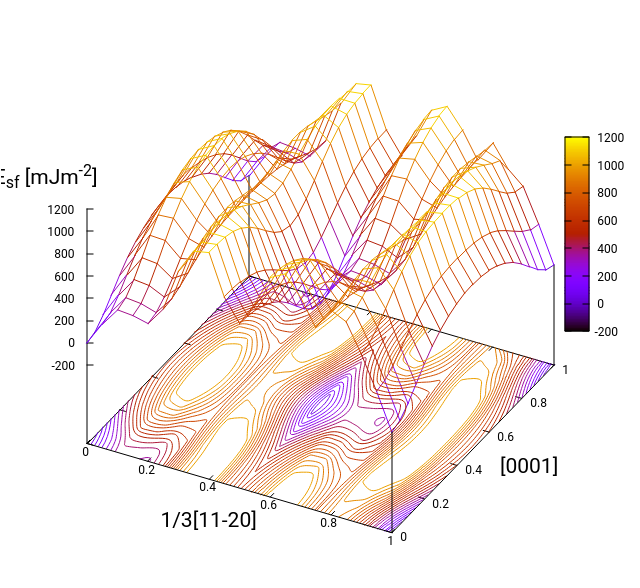
\includegraphics[width=.9\linewidth]{Images/pyramidal_gs_noo_2019-11-08_alat.png}
\end{center}

DFT pseudopot:
\begin{center}
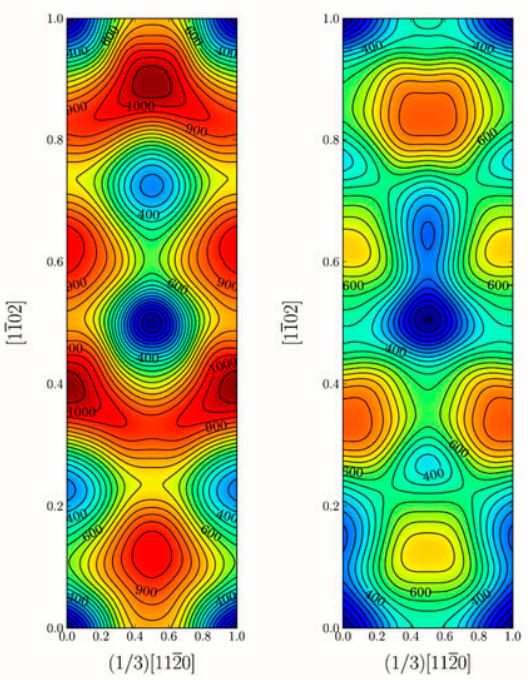
\includegraphics[width=.9\linewidth]{Images/pyramidal_gamma_surface_ready_data_both.png}
\end{center}

\subsection{Data}
\label{sec:org9491dc0}
\href{file:///home/tigany/Documents/ti/final\_model\_2019-11-12/results\_2019-11-09\_muc/gamma\_surfaces/basal/basal\_gs\_noo\_alat\_energies.dat}{basal\(_{\text{gs}}\)\(_{\text{data}}\)}
\href{file:///home/tigany/Documents/ti/final\_model\_2019-11-12/results\_2019-11-09\_muc/gamma\_surfaces/prismatic/prismatic\_gs\_noo\_alat\_energies.dat}{prismatic\(_{\text{gs}}\)\(_{\text{data}}\)}
\href{file:///home/tigany/Documents/ti/final\_model\_2019-11-12/gamma\_surfaces/pyramidal\_results\_2019-11-13/pyramidal\_gamma\_surface\_2019-11-13.dat}{pyramidal\(_{\text{gs}}\)\(_{\text{data}}\)}
\section{Dislocation core structures}
\label{sec:org9246a69}
In the following figures we have the partial differential
displacement maps of dislocations in their initial and final
state. The atoms were relaxed until the root-mean square force
acting on each atom was less than \(1\times 10^-5\) Ryd/Bohr. 

These relaxations can be distinguished by the different initial
positions of the dislocation centre (elastic centre) as following
the paper by Tarrat \cite{Tarrat2009}.

The partial burger's vector seen here is the \(1/6 [11\bar{2}0]\)
dislocation.

One can see that all of the dislocations have dissociated on the
prismatic plane. But there is a difference between initial
positions as to upon which prismatic plane they dissociate on,
from the original. 

Only initial position 2 actually dissociated on a different
prismatic plane to the others. 


There does seem to be a large dissociation distance. 

There is a small energy difference between the dip in the
prismatic gamma surface along the \(1/3 [11\bar{2}0]\)
direction. This means that along that direction, due to the small
relative energy barrier between the trough in the centre of the
gamma surface line and the peaks, so to speak, the dislocation
can dissociate easily along this direction. 

The dissociation distance is consistent between the different
initial positions of the elastic centres. The distance is \(\approx4c =
    35.4\) Bohr \(= 18.7 \AA\).

This is roughly double the distance that is found in the DFT Zr
results by Clouet \cite{Clouet2012}.

\subsection{{\bfseries\sffamily TODO} Dissociation Distance Analysis}
\label{sec:org0e29d56}
Following \cite{Clouet2012}, one can dislocation elasticity theory to
compute the dissociation distance of a dislocation in both the
basal and prism planes.  The energy variation caused by a
dissociation length \(d\) is

\[ \Delta E_{\text{diss}}(d) = - b_i^{(1)}K_{ij}b_j^{(2)}\ln \big( \frac{d}{r_c}
   \big) + \gamma d,  \]

where \(\mathbf{b}^{(i)}\) are the burger's vectors of the dissociated
dislocations.  \(\gamma\) is the corresponding gamma surface energy and
\(K\) is the Stroh matrix. Controlling the dislocation core radius
and the dislocation elastic energy, one can find the equilibrium
dissociation distance as 

\[
   d^{\text{eq}} = \frac{ b_i^{(1)}K_{ij}b_j^{(2) }}{\gamma}
   \]


With the orientation of the simulation cell as, \(U_1 = na \frac{1}{2} [10\bar{1}0]\), \(U_2 = mc [0001]\), 
 \(U_3 =  a \frac{1}{3} [1\bar{2}10]\), one finds the components of
 the Stroh matrix as:

\begin{align}
&K_{11} =& &\frac{1}{2\pi} \big( \bar{C}_{11} + C_{13} \big)
      \sqrt{ \frac{ C_{44} \big( \bar{C}_{11} - C_{13} \big)  }{
	      C_{33} \big( \bar{C}_{11} + C_{13} + 2C_{44} \big)  } 
	   }
\\    
&K_{22 }=& &\sqrt{ \frac{ C_{33} }{ C_{11} }  } K_{11}
\\
&K_{33} =& &\frac{1}{2\pi} \sqrt{ \frac{1}{2} C_{44} \big( C_{11} - C_{12} \big)  }_{}
\end{align}

here, \(\bar{C}_{11} = \sqrt{ C_{11}C_{33} }\).


From the gamma surface, for the basal plane one expects a
dissociation of \(1/3[1\bar{2}10] = 1/3[1\bar{1}00] +
    1/3[0\bar{1}10]\). Then dissociation length in the basal plane is
given by 

\[
    d_{\text{b}}^{\text{eq}} = \frac{ ( 3K_{33} - K_{11} ) a^2 }{ 12 \gamma_{\text{b}} } 
    \]

For the prism plane the \(1/3[1\bar{2}10]\) dislocation can
dissociate into \(1/6[1\bar{2}10] \pm \alpha(c/a)[0001]\) where the
parameter \(\alpha\) controls the position of the stacking fault minimum
along the [0001] direction. Only in interatomic potentials like
the EAM, do we find that \(\alpha = 0.14\). 

The dissociation length is 

\[
    d_{\text{p}}^{\text{eq}} = \frac{ ( K_{33}a^2 - 4 \alpha^2 K_{22} c^2 ) }{ 4 \gamma_{p} }
    \]


\subsection{{\bfseries\sffamily TODO} Disregistry Analysis}
\label{sec:org216bc17}
Look into the theory of dissociation distance in Clouet paper
\cite{Clouet2012}


Disregistry given by the Peierls-Nabarro model. Analytic
expression given in Hirth and Lothe \cite{anderson2017theory}.

Disregistry \(D(x)\) is defined as the displacement difference
between the atoms in the plane just above and those just below the
dislocation glide plane. The derivative of this function \(\rho(x) = \partial
    D / \partial x\) corresponds to the dislocation density.


\[
    D_{\text{dislo}} = \frac{b}{2\pi} 
    \Bigg\{ \arctan \bigg[  \frac{x - x_0 - d/2}{ \zeta } \bigg] +
           \arctan \bigg[  \frac{x - x_0 + d/2}{ \zeta } + \frac{\pi}{2} \bigg]
	   \Bigg\}
    \]

Given \(x_0\) is the dislocation position, \(d\) is dissociation
length and \(\zeta\) is the spreading of each partial dislocation. 

\begin{align*}
  D_{L} &= &\sum_{n = -\infty}^{\infty}  &D_{\text{dislo}} (x - nL) \\
     &= &\frac{ b }{ 2\pi } 
        \Bigg \{ 
         &\arctan \bigg[ 
            \frac{ 
                  \tan \big( \frac{\pi}{L} [x - x_0 - d/2] \big)
                 }{ 
                 \tanh \big( \frac{\pi\zeta}{L} \big)
                  } \bigg]
       + \pi\bigg\lfloor 
       	 \frac{x - x_0 - d/2}{ \zeta } + \frac{1}{2}
       \bigg\rfloor \\
   & &+
         &\arctan \bigg[ 
            \frac{ 
                  \tan \big( \frac{\pi}{L} [x - x_0 + d/2] \big)
                 }{ 
                 \tanh \big( \frac{\pi\zeta}{L} \big)
                  } \bigg]
       + \pi \bigg\lfloor 
       	 \frac{x - x_0 + d/2}{ \zeta } + \frac{1}{2}
       \bigg\rfloor    \Bigg\},
\end{align*}

where \(\lfloor \cdot \rfloor\) is the floor function. 

For an array of dislocations in the S arrangement, \(D(x) = D_L(x)\),
with \(L = mc\), where \(m\) is the number of repeated unit cells in
the \(U_2\) direction. 

Here, \(U_1 = na \frac{1}{2} [10\bar{1}0]\), \(U_2 = mc [0001]\), 
\(U_3 =  a \frac{1}{3} [1\bar{2}10]\).

This procedure therefore allows us to determine the location of
the dislocation center. For all interaction models, we find that
this center lies in between two (0001) atomic planes. One can see
in Fig. 6 of \cite{Clouet2012} that this position corresponds to a
local symmetry axis of the differential displacement map. This is
different from the result obtained by Ghazisaeidi and Trinkle
\cite{Ghazisaeidi2012} in Ti where the center of the screw
dislocation was found to lie exactly in one (0001) atomic plane.

\newpage


\subsection{IP1}
\label{sec:orge3d23f7}
\begin{center}
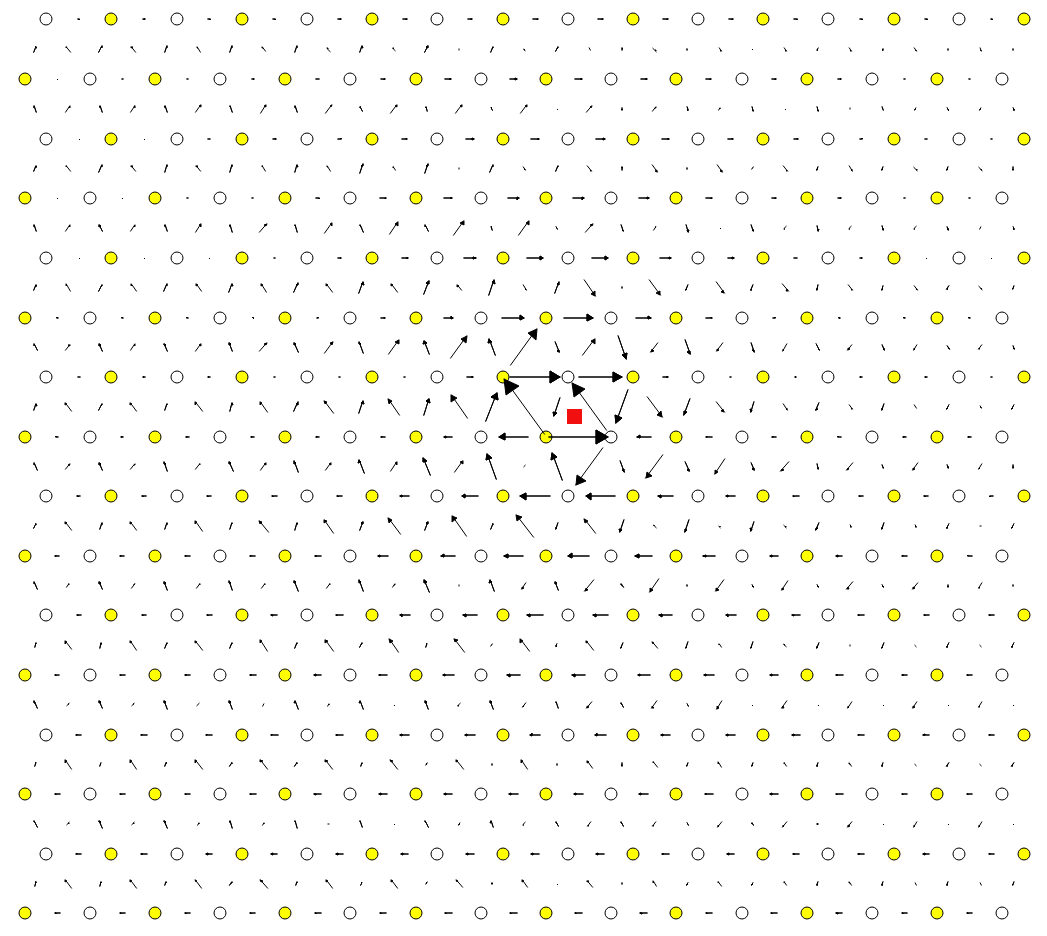
\includegraphics[width=0.7\textwidth]{Images/final_model_IP1_partial_dd_initial.png}
\end{center}
\begin{center}
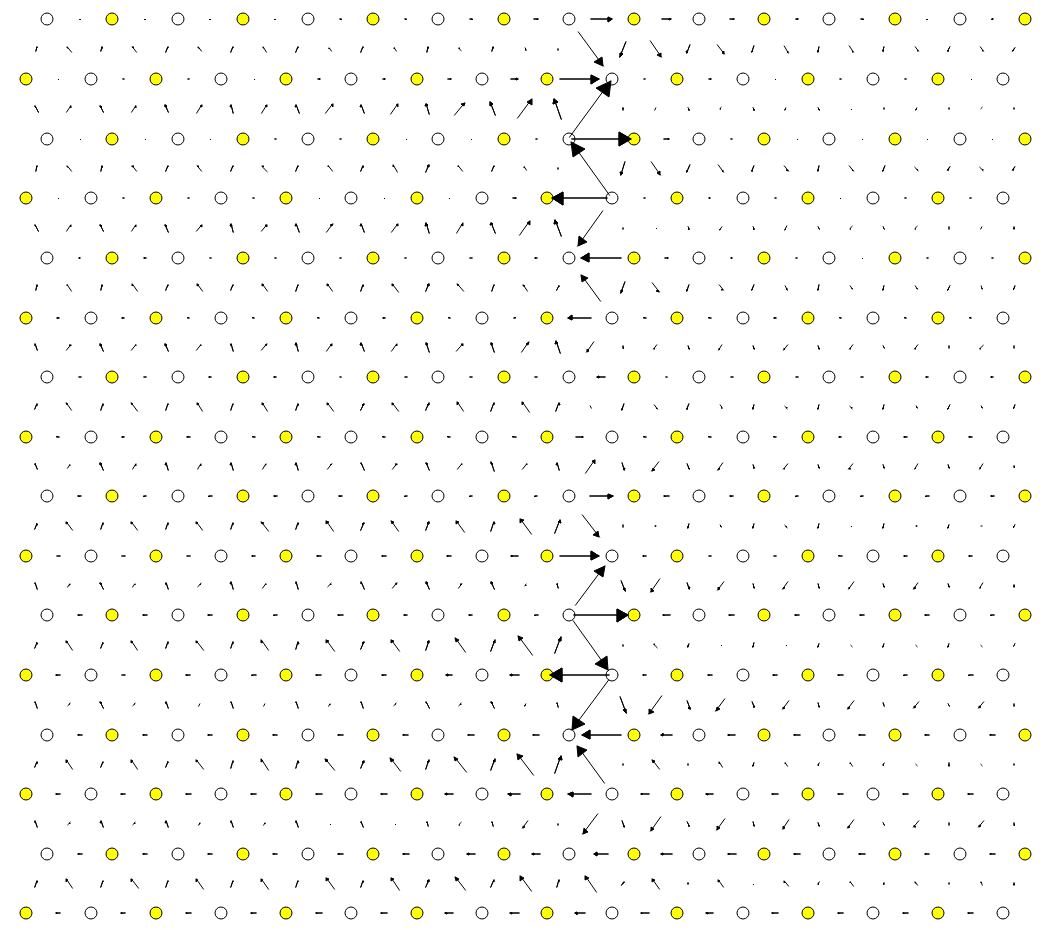
\includegraphics[width=0.7\textwidth]{Images/final_model_IP1_partial_dd_final.png}
\end{center} 

\subsection{IP2}
\label{sec:org2a6f9b4}
\begin{center}
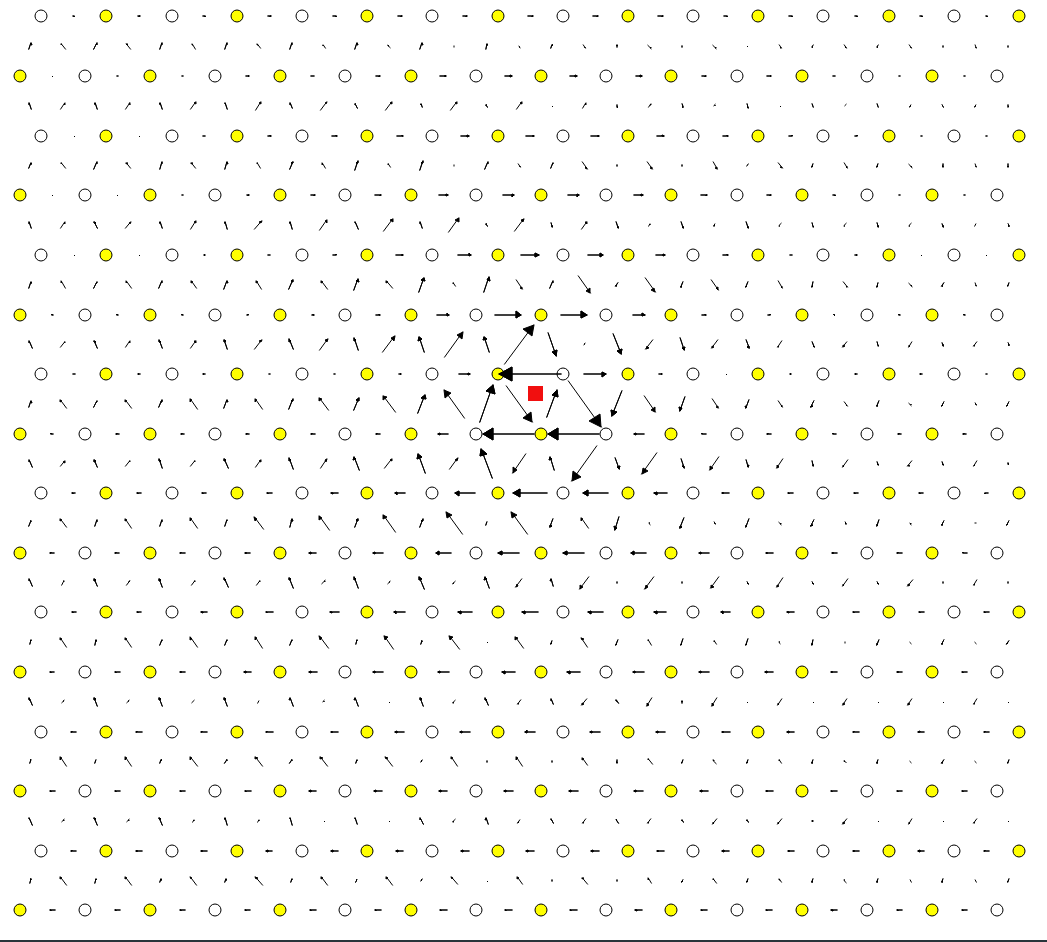
\includegraphics[width=0.7\textwidth]{Images/final_model_IP2_partial_dd_initial..png}
\end{center}
\begin{center}
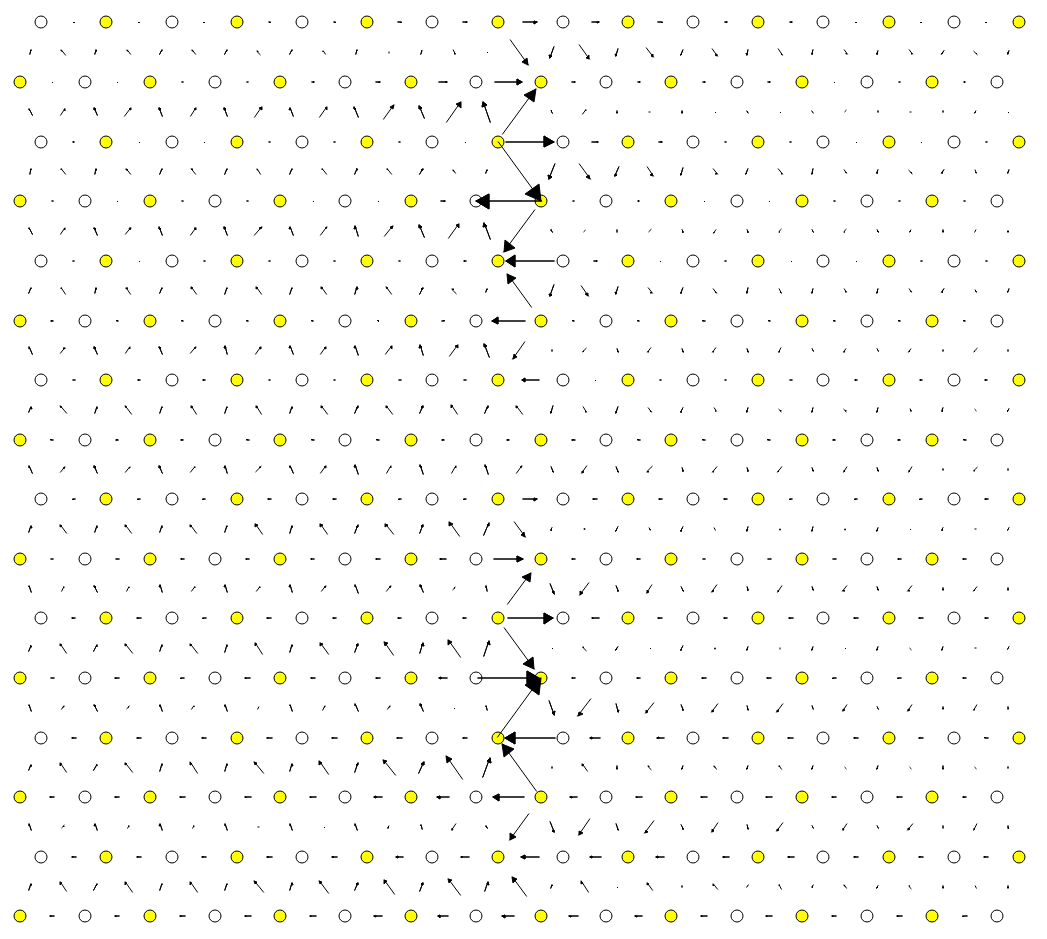
\includegraphics[width=0.7\textwidth]{Images/final_model_IP2_partial_dd_final.png}
\end{center}
\subsection{IP3}
\label{sec:org388131e}
\begin{center}
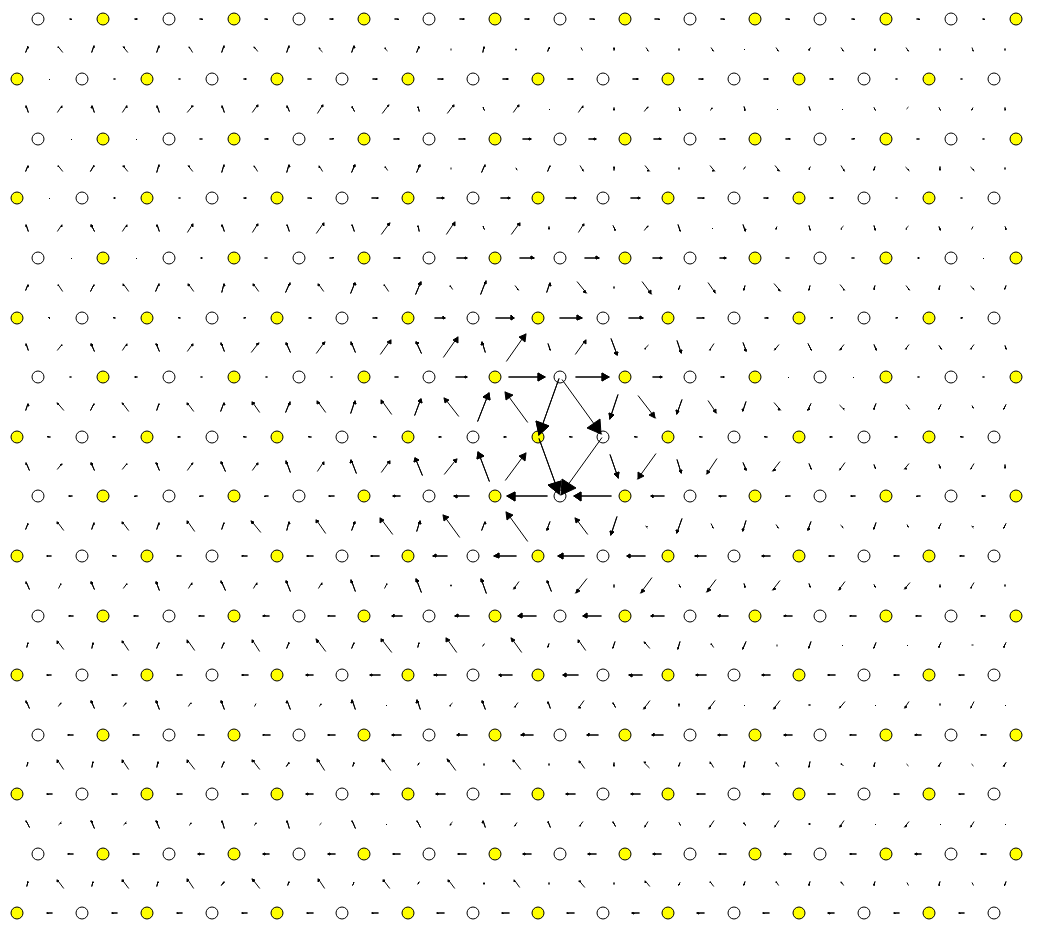
\includegraphics[width=0.7\textwidth]{Images/final_model_IP3_partial_dd_initial.png}
\end{center}
\begin{center}
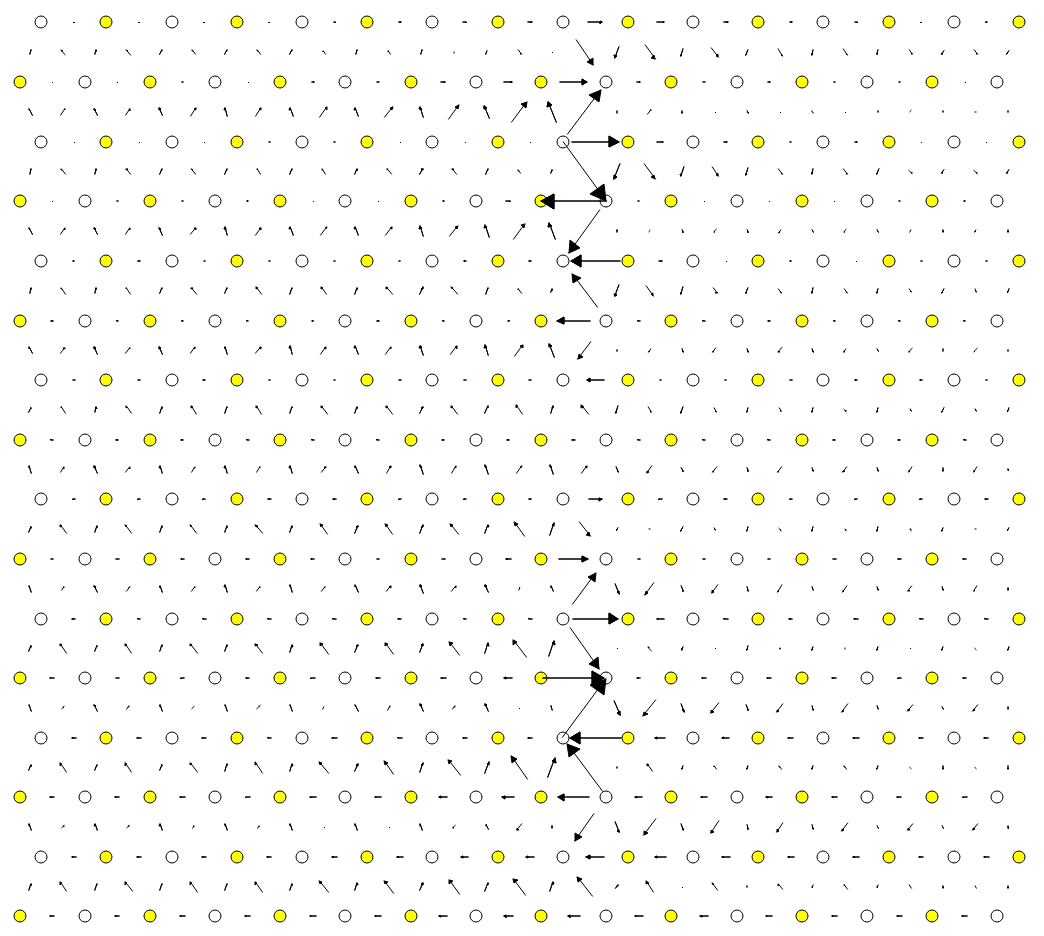
\includegraphics[width=0.7\textwidth]{Images/final_model_IP3_partial_dd_final.png}
\end{center}
\subsection{IP4}
\label{sec:org93a356f}
\begin{center}
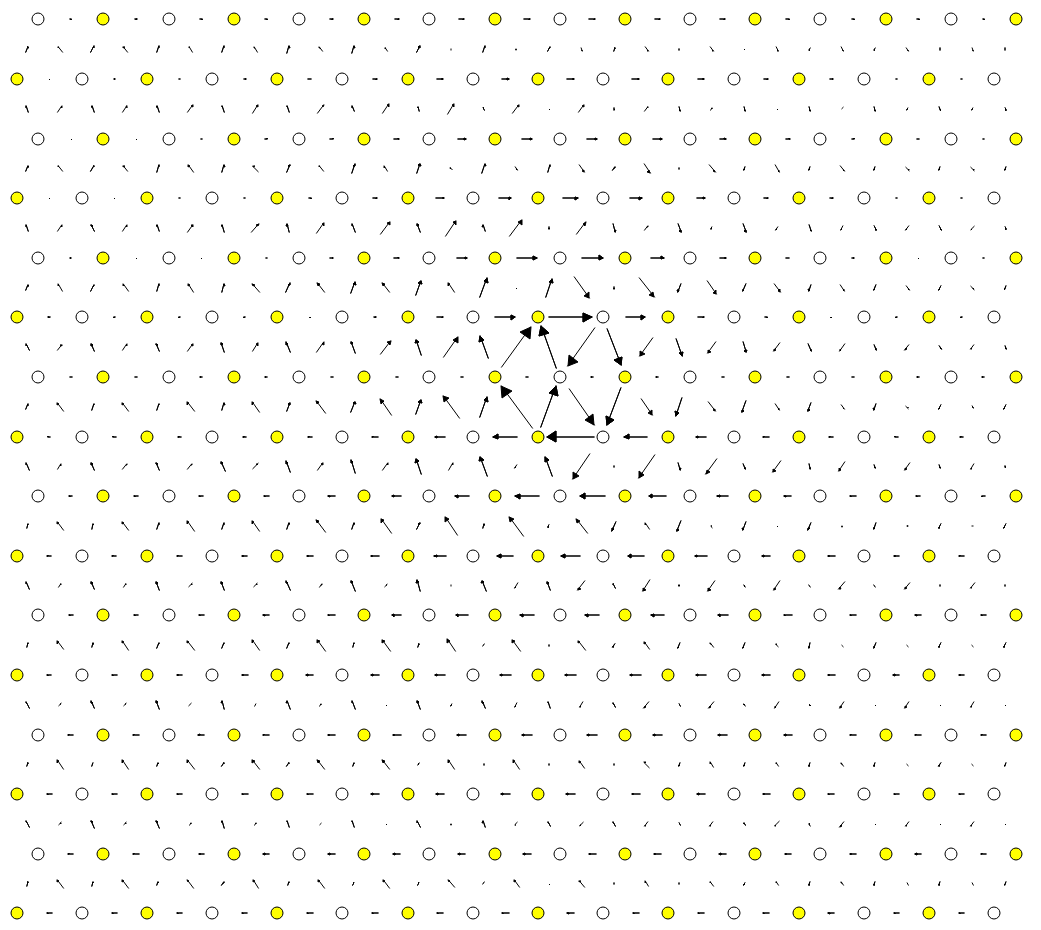
\includegraphics[width=0.7\textwidth]{Images/final_model_IP4_partial_dd_initial.png}
\end{center}
\begin{center}
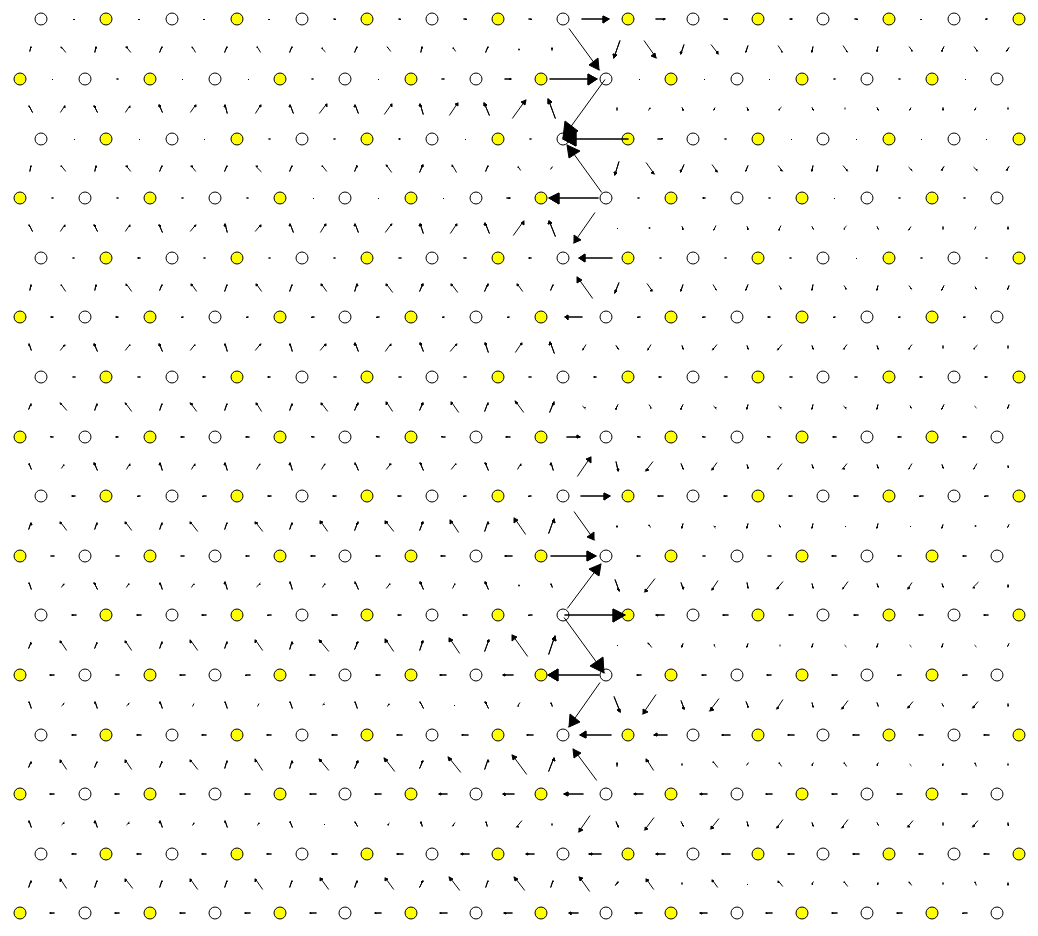
\includegraphics[width=0.7\textwidth]{Images/final_model_IP4_partial_dd_final.png}
\end{center}
\subsection{IP5}
\label{sec:org3806fd4}
\begin{center}
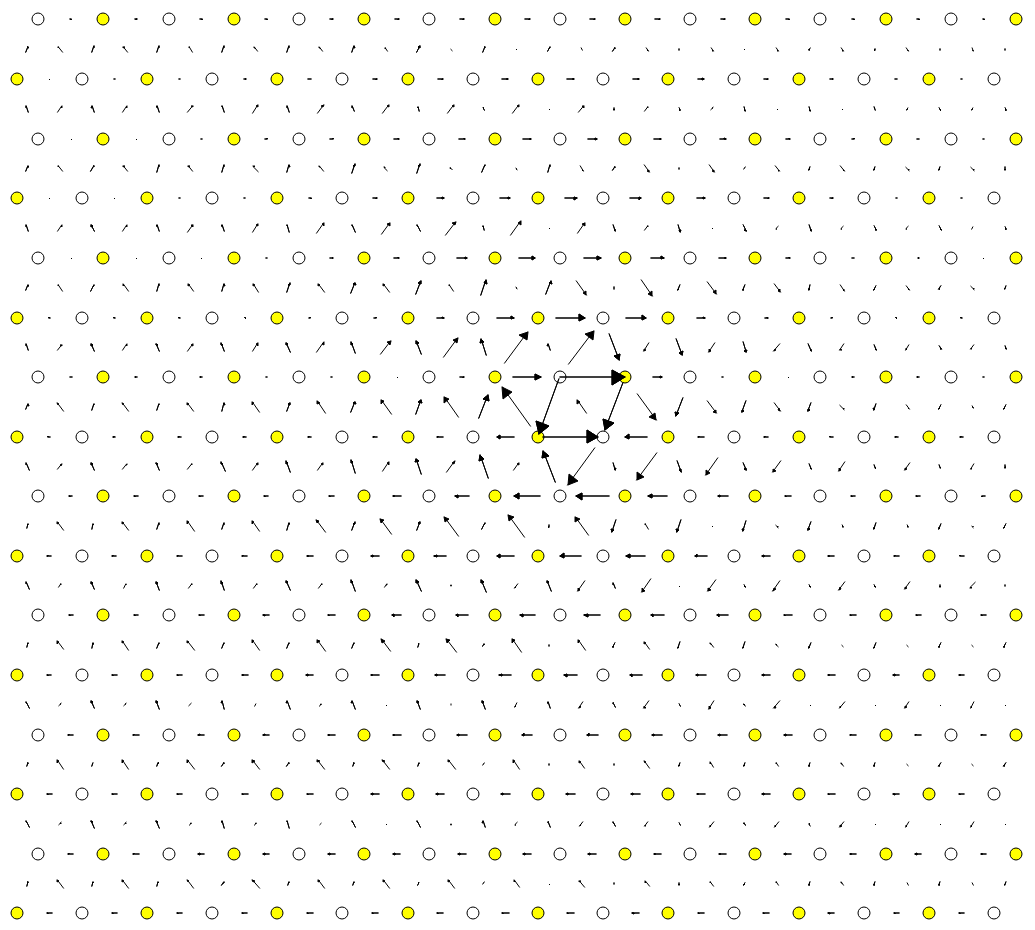
\includegraphics[width=0.7\textwidth]{Images/final_model_IP5_partial_dd_initial.png}
\end{center}
\begin{center}
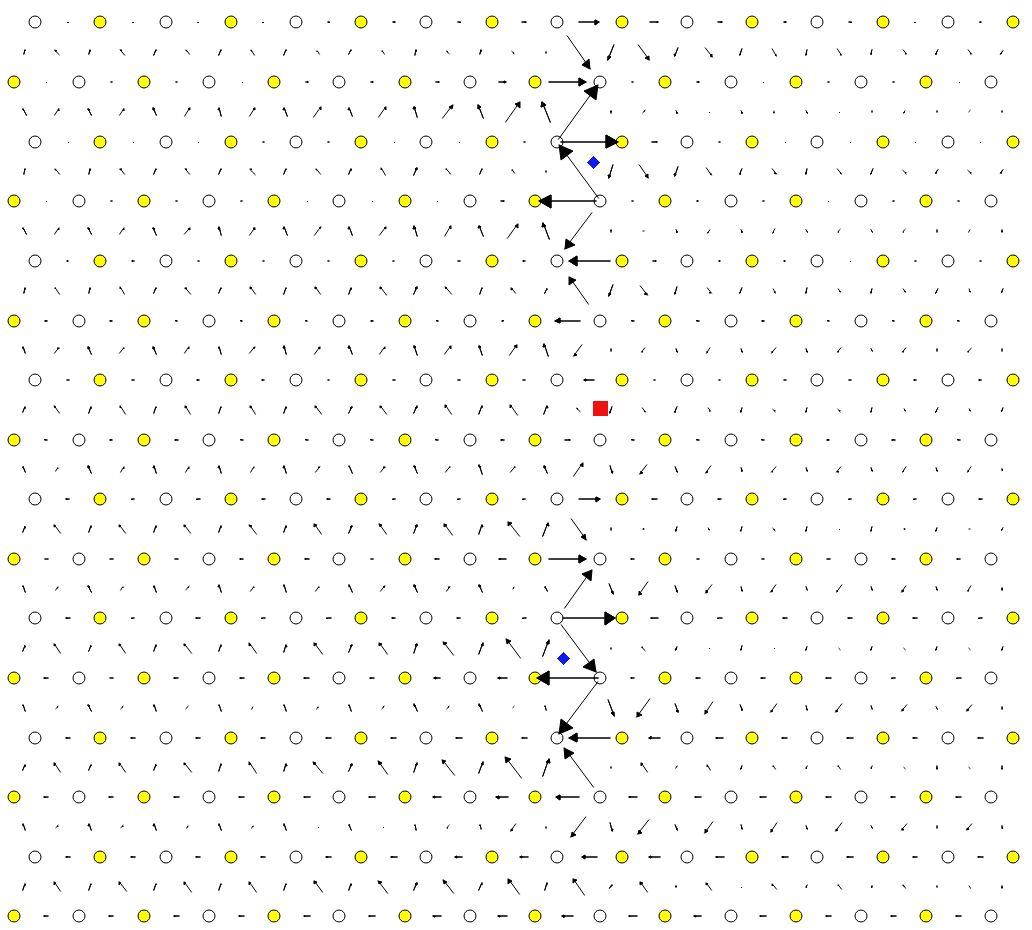
\includegraphics[width=0.7\textwidth]{Images/final_model_IP5_partial_dd_final.png}
\end{center}

\subsection{Ghazisaeidi Results for comparison}
\label{sec:orgfa7c439}

\begin{center}
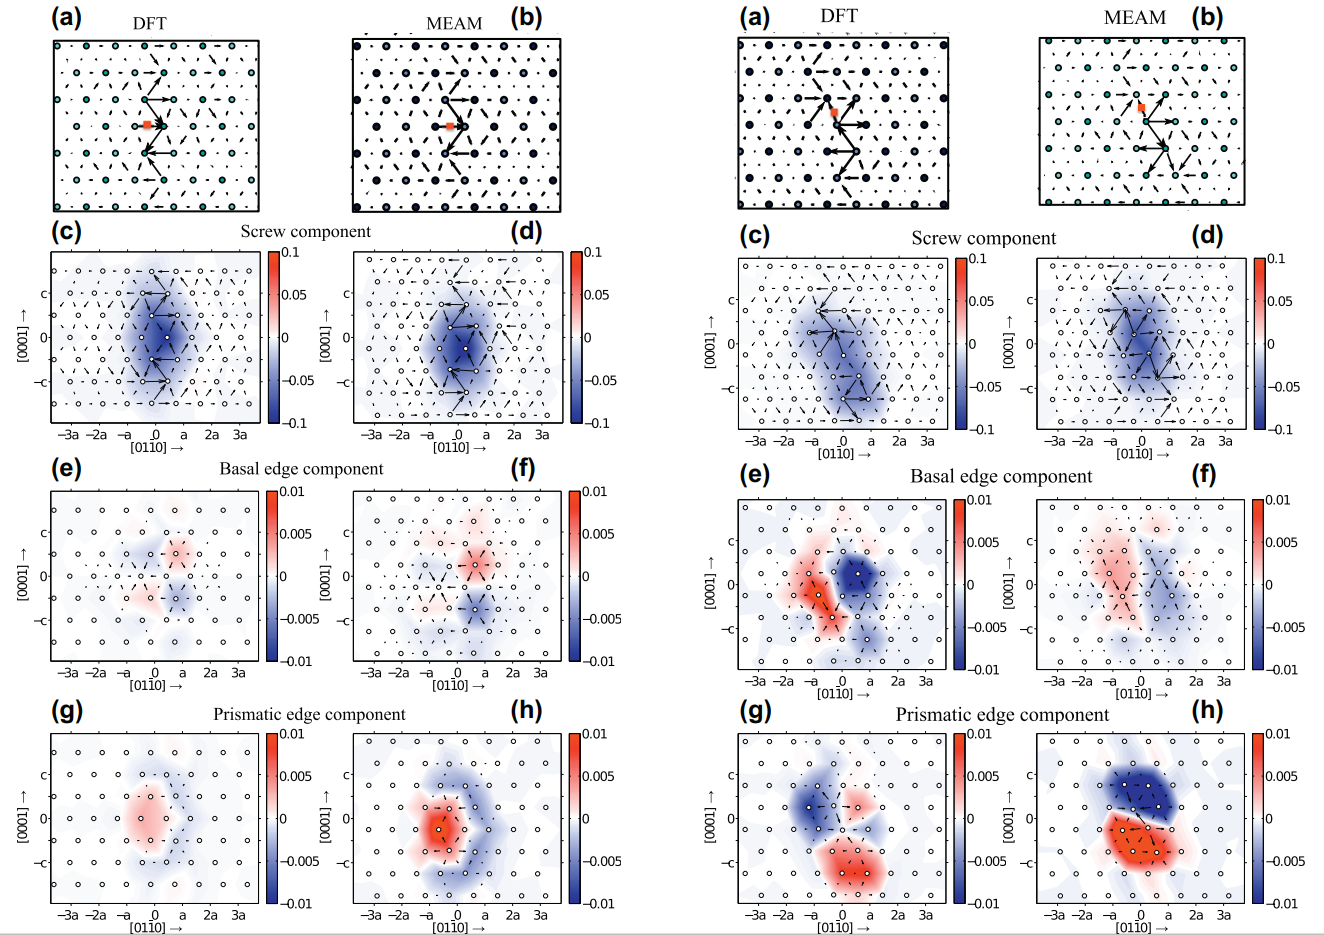
\includegraphics[width=0.7\textwidth]{Images/ghazisaiedi-trinkle-scew-dislocation-core-prism-symm-asymm.png}
\end{center}

\subsection{Peierls Stress}
\label{sec:orgf7869bf}

By straining lattice and incrementally increasing the strain, one
can find the minimum stress necessary to move a dislocation from one
Peierls valley to the next. 

\subsubsection{xy strain 0.03}
\label{sec:org8acfd35}

Here the \(\alpha\) parameter is 0.03. 

This means that the stress necessary to move the dislocation is 

\begin{align*}
\sigma_{12} &= C_{1212}\varepsilon_{12} \\
    &= 2C^{\text{Voigt}}_{66 }\varepsilon_6^{\text{Voigt}} \\
    &= ( C_{11}- C_{12}) \varepsilon_6^{\text{Voigt}} \\
    &= 76.59 \times 0.03 \\ 
    &= 2.31 GPa\ 
\end{align*}

\begin{center}
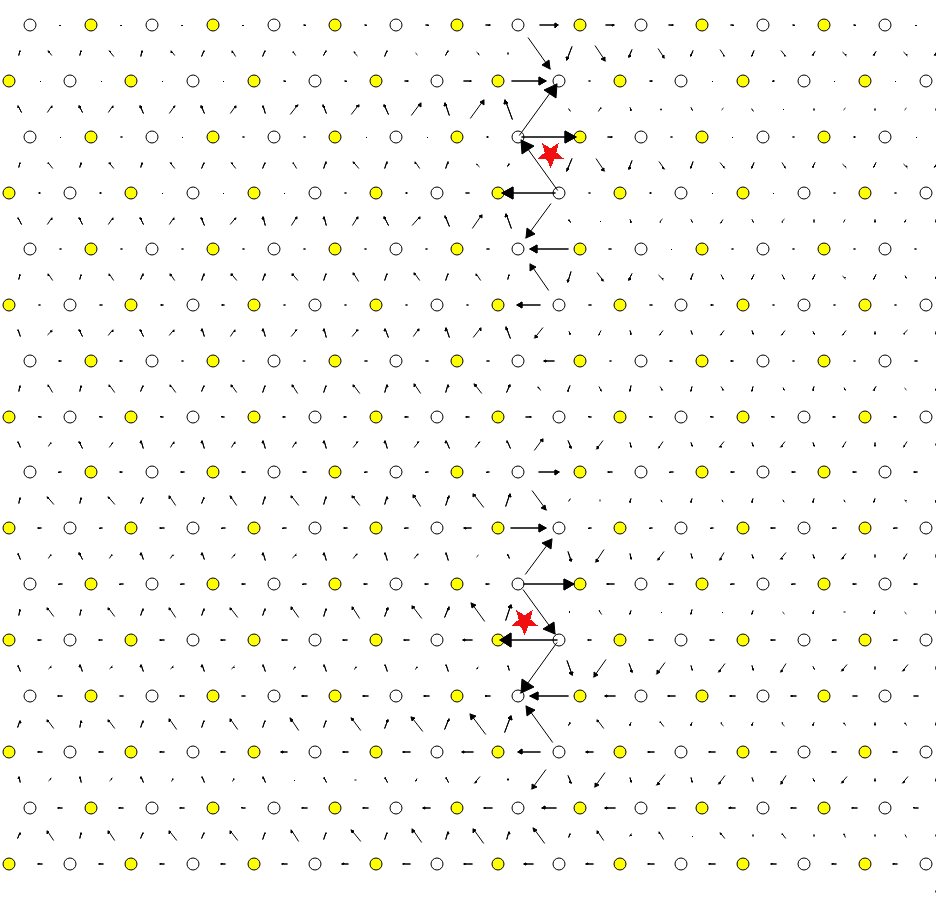
\includegraphics[width=0.7\textwidth]{Images/final_model_peierls_xy_0.03_initial_partials.png}
\end{center}
\begin{center}
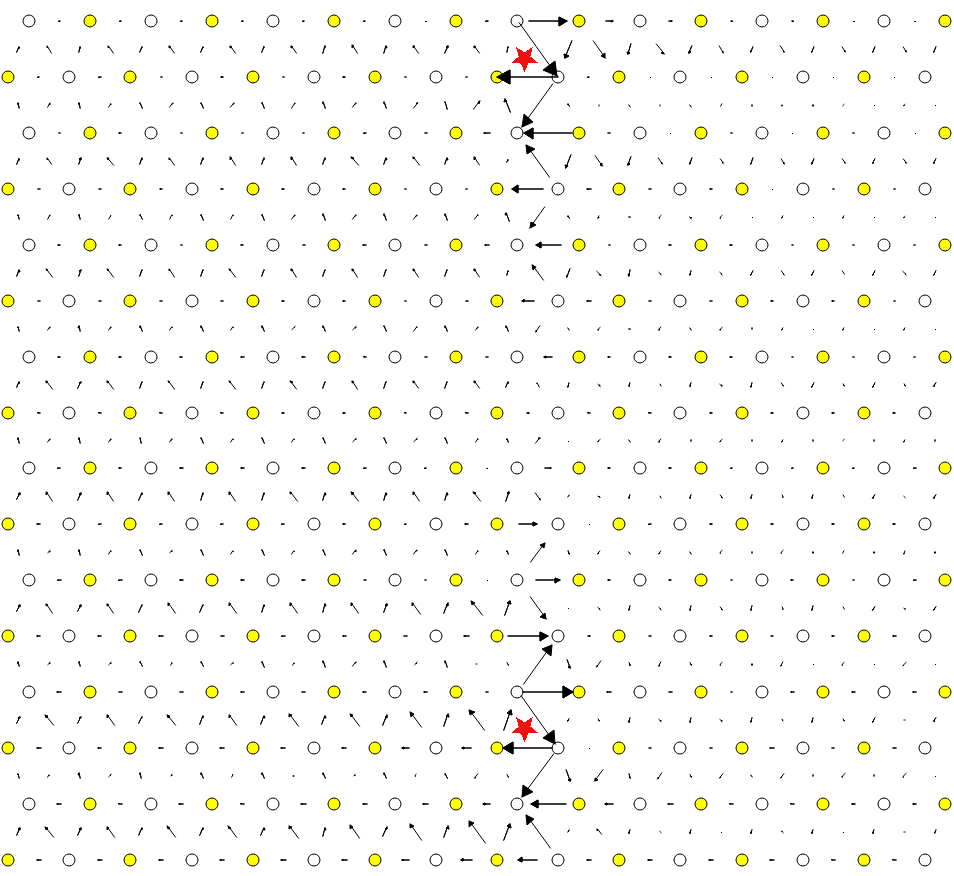
\includegraphics[width=0.7\textwidth]{Images/final_model_peierls_xy_0.03_final_partials.png}
\end{center}


\subsection{Data}
\label{sec:orgfd7559c}
\href{file:///home/tigany/Documents/ti/final\_model\_2019-11-12/results\_2019-11-09\_muc/IP1-oo\_19-11-09--04-46-00.log}{IP1}
\href{file:///home/tigany/Documents/ti/final\_model\_2019-11-12/results\_2019-11-09\_muc/IP2-oo\_19-11-09--04-46-00.log}{IP2}
\href{file:///home/tigany/Documents/ti/final\_model\_2019-11-12/results\_2019-11-09\_muc/IP3-oo\_19-11-09--04-46-00.log}{IP3}
\href{file:///home/tigany/Documents/ti/final\_model\_2019-11-12/results\_2019-11-09\_muc/IP4-oo\_19-11-09--04-46-00.log}{IP4}
\href{file:///home/tigany/Documents/ti/final\_model\_2019-11-12/results\_2019-11-09\_muc/IP5-oo\_19-11-09--04-46-00.log}{IP5}

\subsection{Directory of the results}
\label{sec:orgde5014f}
\url{file:///home/tigany/Documents/ti/2019-09-11\_final\_model/tbe/dislocations/2019-11-08\_no\_omega\_ordering\_ec\_latpar/}
\url{file:///home/tigany/Documents/ti/final\_model\_2019-11}

\section{BOP}
\label{sec:org4fa19fa}

\subsection{4 recursion levels}
\label{sec:org4ba23d1}

kbT = 0.1

>> Lattice parameters:

> hcp
\begin{center}
\begin{tabular}{ll}
a & 2.901660  \AA{}\\
c & 4.747485  \AA{}\\
etot & -18.342162  eV\\
\end{tabular}
\end{center}

> omega
\begin{center}
\begin{tabular}{ll}
a & 7.917318  \AA{}\\
c & 2.749892 \AA{}\\
etot & -17.458700 eV\\
\end{tabular}
\end{center}

Omega is still not as stable as hcp as expected from model. 


>> Elastic Constants

\begin{center}
\begin{tabular}{lrr}
Quantity & calc. (10\(^{\text{11}}\) Pa) & exp. (10\(^{\text{11}}\) GPa)\\
\hline
C11 & 1.781 & 1.761\\
C12 & 0.738 & 0.868\\
C13 & 0.611 & 0.682\\
C33 & 1.969 & 1.905\\
C44 & 0.285 & 0.508\\
C66 & 0.522 & 0.450\\
K & 1.050 & 1.101\\
R & 0.669 & 0.618\\
H & 0.558 & 0.489\\
\end{tabular}
\end{center}

\section{Bibliography}
\label{sec:org9beaf5f}
\label{org842ba38}

\bibliographystyle{unsrt}
\bibliography{bibliography/org-refs}
\end{document}